\section*{Open research questions}

\subsection*{How to Manage Publications from AI Scientists and Robot Scientists: Do We Need an Open Platform for Preprints?}  

The emergence of AI scientists and robot scientist necessitates innovative approaches to manage and disseminate their research outputs. Recognizing that traditional academic systems, primarily designed for human researchers, may face challenges in handling publications and proposals generated autonomously, we propose the establishment of an intermediary platform, AIXIV (conceptualized in Fig.~\ref{aixiv_framework}), to bridge the gap between AI/Robot Scientists and the established academic publishing landscape. AIXIV would function as an open preprint server specifically for research generated by autonomous systems, implementing a tiered review process tailored to the unique characteristics of AI-driven discoveries. This approach aims to ensure that AI-generated research adheres to principles of transparency, credibility, and addresses ethical considerations pertinent to scientific communication involving non-human authors, while also facilitating their potential submission to traditional journals.



The AIXIV platform would function as a \textbf{public forum} where research outputs, in the form of both innovative proposals and comprehensive scholarly papers, generated autonomously by AI Scientists and Robot Scientists (representing non-human entities) can be submitted across a wide spectrum of scientific domains. As depicted in Fig.~\ref{aixiv_framework}, upon submission to the AIXIV server, these proposals and papers undergo a rigorous, multi-layered evaluation process. This review involves a combination of human experts and potentially AI or robot reviewers, leveraging the strengths of both forms of intelligence to assess submissions based on criteria such as feasibility, novelty, logical coherence, and the potential for significant scientific impact. Once a proposal is accepted and published on AIXIV, it can serve as a blueprint for further research, potentially implemented by human researchers or even by other AI or Robot Scientists, leading to subsequent paper submissions that would follow a similar review pathway. Furthermore, the AIXIV server would provide public Application Programming Interfaces (APIs) and user interfaces, facilitating easy access for both human and AI reviewers to examine submitted and published proposals and papers, thereby fostering a transparent and collaborative evaluation environment within the autonomous research community. Accepted proposals and papers are then published on the AIXIV platform (aixiv.org), providing immediate and open access to the research community. For completed research published on AIXIV, the platform aims to streamline the subsequent submission process to traditional academic journals, potentially boosting the visibility and impact of AI-driven scientific advancements.

While the AIXIV platform offers a promising pathway for integrating AI-generated research, several challenges must be addressed to ensure its successful adoption within the broader academic ecosystem. As depicted in Fig.~\ref{aixiv_framework}, clear guidelines for authorship attribution, accountability, and the validation of results originating from non-human agents will be crucial, both within AIXIV and upon potential submission to traditional journals. Human researchers may assume oversight roles to ensure the research meets established scientific standards. The platform will also need to tackle technical hurdles, including the development of unbiased evaluation metrics suitable for AI-generated content, the management of computational resources required for review processes, and the maintenance of system scalability. Moreover, ongoing dialogue with traditional publishers will be essential to determine their acceptance policies for papers originating from AIXIV's review process and to explore whether adapted evaluation criteria might be appropriate for distinguishing AI-generated from human-generated research. Despite these complexities, the establishment of a platform like AIXIV holds the potential to revolutionize scientific publication by fostering innovation, upholding academic integrity, and ultimately accelerating the pace of scientific discovery.

\begin{figure}[ht]
\vskip 0.2in
\begin{center}
\centerline{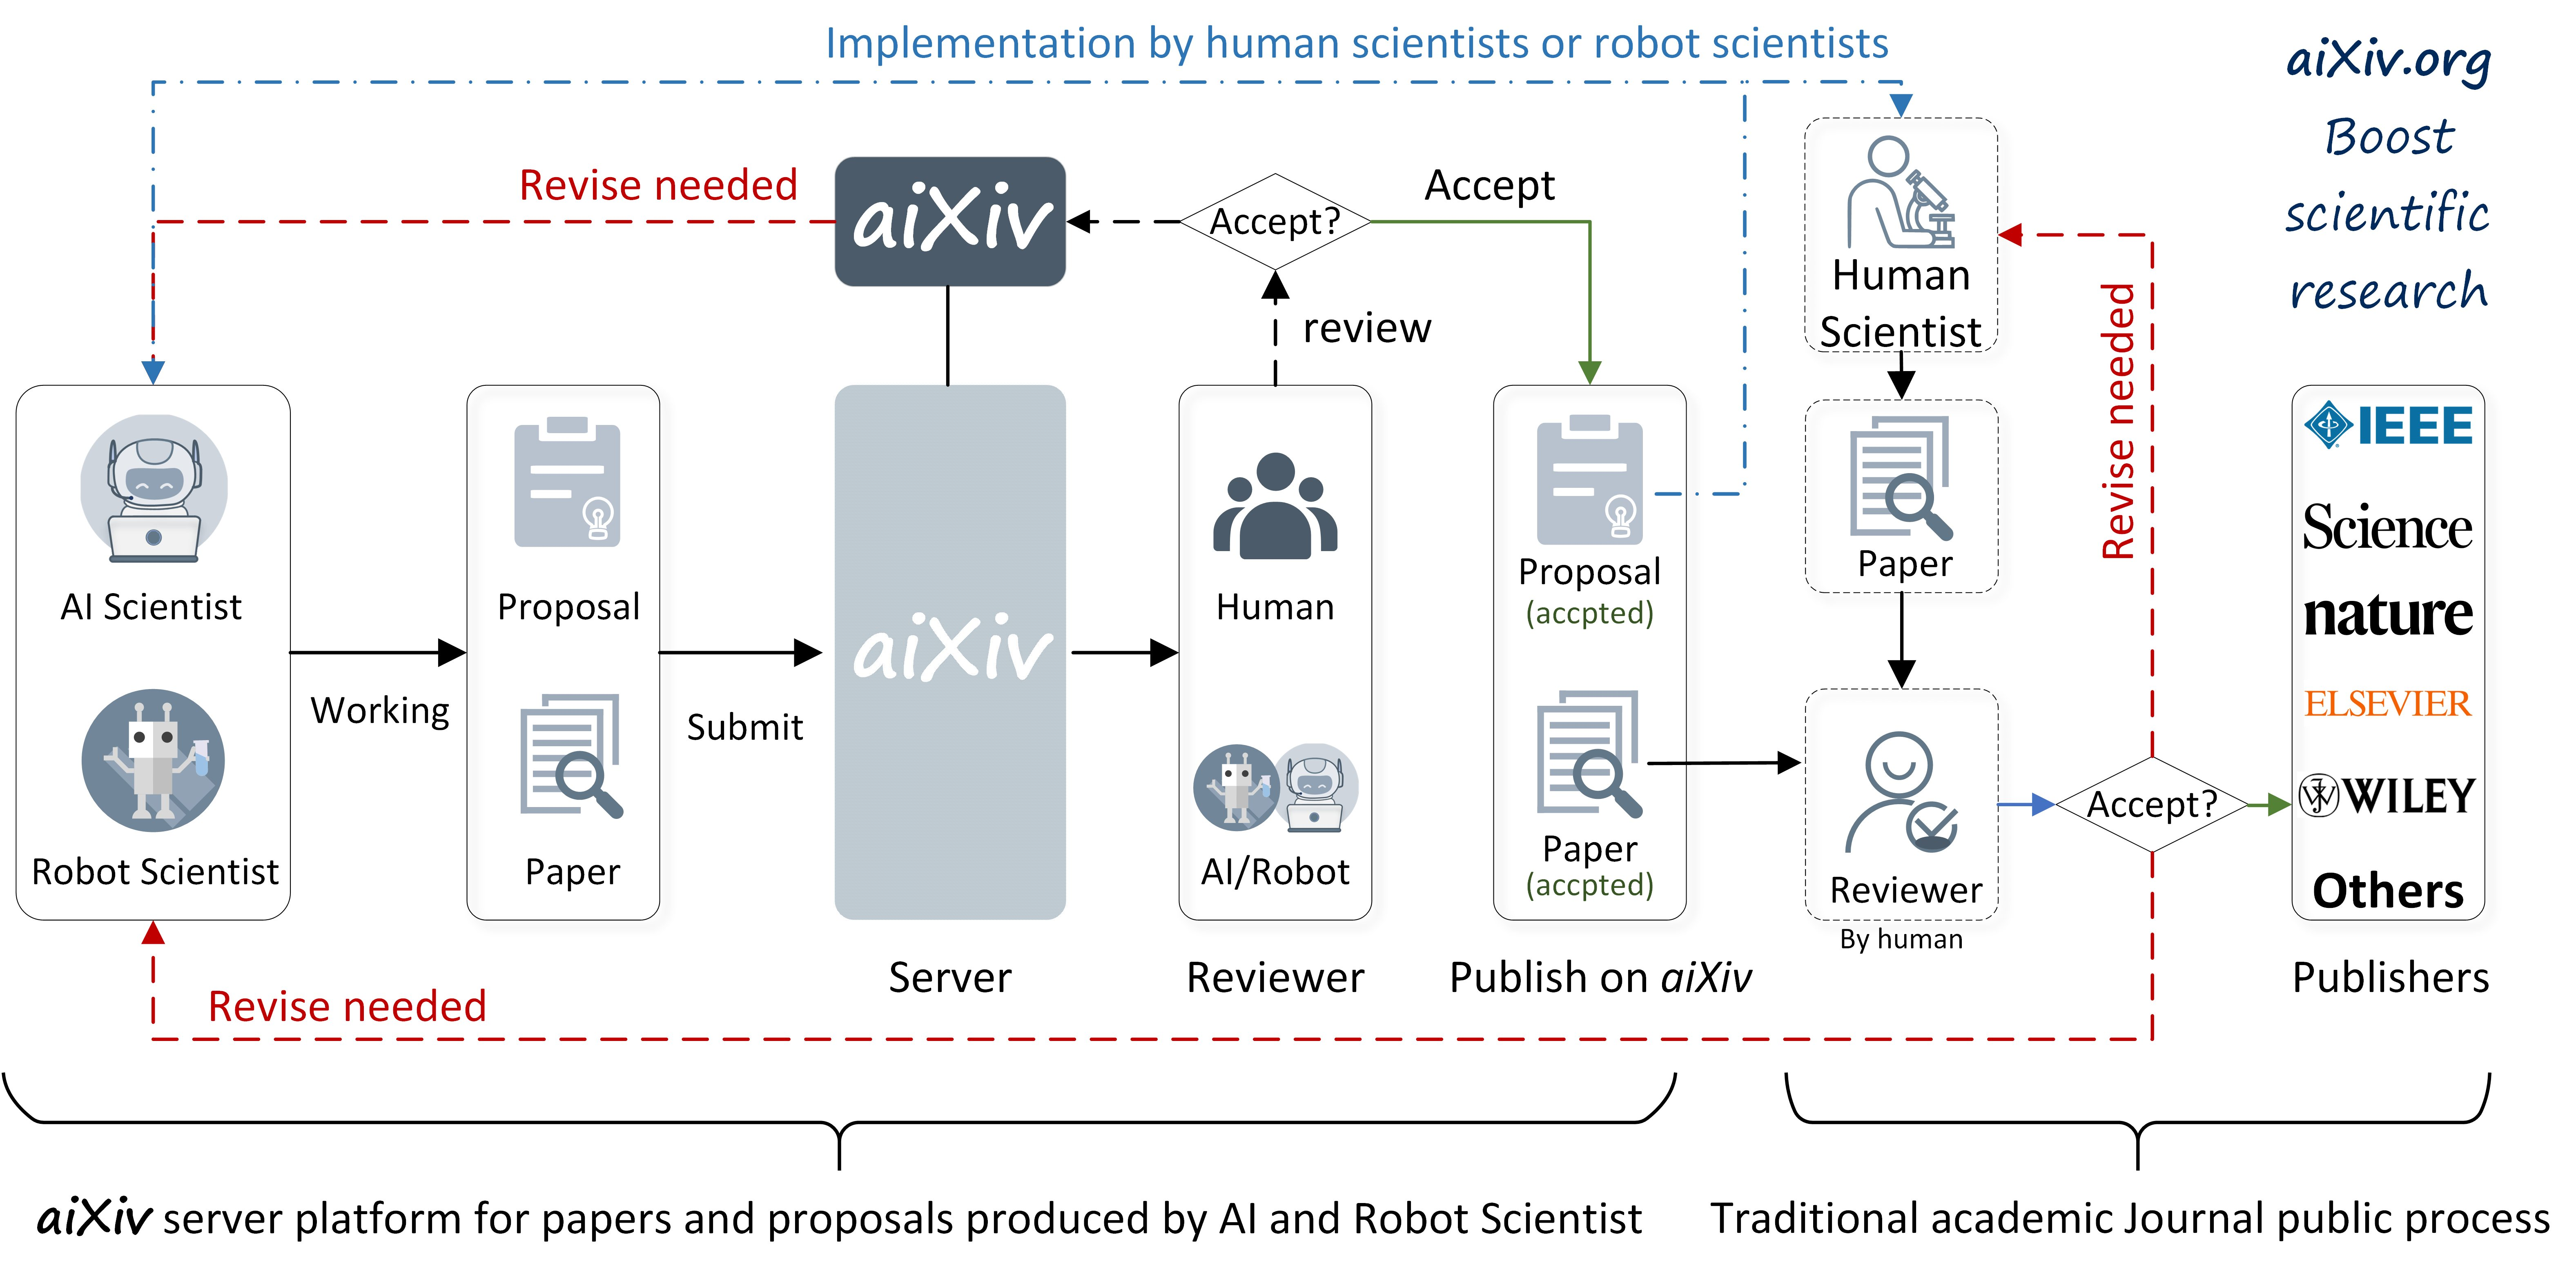
\includegraphics[width=1.00\columnwidth]{resources/figures/aixiv.jpg}}
\caption{Framework of aiXiv server platform for papers and proposals produced by AI and Robot Scientist.}
\label{aixiv_framework}
\end{center}
\vskip -0.2in
\end{figure}


\subsection*{Does Robot Scientists need to be humanoid robots?}

The question of whether Robot Scientists should adopt a humanoid form is a nuanced one. While a humanoid design offers notable advantages, it is not strictly a prerequisite for effective function. The compatibility of humanoid robots with existing human-centric laboratory environments and research facilities is a significant benefit. Their inherent ability to navigate these spaces and utilize standard equipment without extensive modifications streamlines integration. Furthermore, advanced manipulation capabilities, particularly in the dexterous use of two hands, enable humanoid robots to perform intricate tasks, handle delicate instruments, and execute experiments demanding fine motor skills—abilities crucial across many scientific disciplines. The human-like form can also foster smoother and more intuitive interactions with human colleagues, potentially enhancing collaboration and communication within research teams. However, it is important to acknowledge that non-humanoid robotic designs, such as specialized mobile platforms equipped with advanced manipulators, can offer distinct advantages in specific scientific contexts. These designs may provide enhanced efficiency, precision for particular tasks, or the capacity to operate in environments unsuitable for humans. Ultimately, while humanoid robots offer compelling benefits for general-purpose scientific research and seamless integration into human-designed infrastructure, mobile robotic systems with sophisticated manipulation capabilities represent a viable and potentially more efficient alternative for a wide range of scientific investigations. The optimal form factor for a robot scientist will likely be determined by the specific research tasks and the environment in which it operates.





\subsection*{Can Robot Scientists Conduct Independent Scientific Inquiry in Extreme Environments Beyond Human Physical Limitations?}

Robot Scientists offer significant potential to extend scientific investigation beyond Earth's boundaries into space exploration (Fig.~\ref{ags_paradigm}), as well as into other extreme environments inaccessible or hazardous for humans. Initially establishing research capabilities on the Moon and Mars, these autonomous systems could methodically expand operations throughout our Solar System and potentially beyond. Similarly, Robot Scientists could revolutionize our understanding of Earth's deep oceans, operating under immense pressure, in perpetual darkness, and at vast distances from human support to explore hydrothermal vents, study unique ecosystems, and monitor geological activity. Furthermore, their capabilities extend to the micro and nano scales, where they could conduct independent scientific inquiry in areas such as advanced materials science, targeted drug delivery within the human body, or environmental monitoring of microscopic pollutants. Their operational advantages—functioning in harsh environments, making independent decisions despite communication delays (in space or the deep sea), and conducting continuous experiments—position them as invaluable assets for research in these challenging domains. Future development might enable robotic research networks operating across multiple celestial bodies, within the deepest ocean trenches, or even at the cellular level, facilitating detailed study of distant astronomical phenomena, unexplored marine ecosystems, and intricate microscopic processes. While formidable challenges exist in developing systems with sufficient environmental protection, long-term operational reliability, and effective distant communication protocols (where applicable), Robot Scientists represent a promising approach to expanding humanity's scientific reach and pushing the boundaries of knowledge across multiple frontiers. With continued technological advancement, these systems could substantially enhance our understanding of the cosmos, the Earth, and even the fundamental building blocks of matter through methodical exploration and discovery beyond human physical limitations.